%!LW recipe=latexmk
% !TEX root = main.tex
%# -*- coding:utf-8 -*-

\PassOptionsToPackage{quiet}{fontspec}
\PassOptionsToPackage{fontset=fandol}{ctex}
\PassOptionsToPackage{dvipsnames}{xcolor}
\documentclass[10pt,aspectratio=169]{beamer}
\usepackage{pkubeamer}

\usepackage{booktabs}
\usepackage{tabularx}
\usepackage{array}
\usepackage{ragged2e}
\usepackage{amsmath}
\usepackage{amssymb}
\usepackage{stmaryrd}
\usepackage{mathpartir}
\usepackage{pifont}
\usepackage{tikz}
\usetikzlibrary{fit,arrows.meta,backgrounds,positioning,calc,shapes.geometric,decorations.pathreplacing}
\usepackage{listings}
% \usepackage{listings-ocaml}
% \usepackage{listings-c}

% Shared mathematical notation and presentation helpers.

% Logic.
\newcommand{\IProp}{\mathsf{iProp}}
\newcommand{\Heap}{\mathsf{Heap}}
\newcommand{\PropCat}{\mathbf{Prop}}
\newcommand{\Later}{\mathord{\triangleright}}
\newcommand{\Always}{\mathord{\Box}}
\newcommand{\Sep}{\mathbin{*}}
\newcommand{\Wand}{\mathbin{-\!*}}
\newcommand{\Entails}{\mathrel{\vdash}}
\newcommand{\Sem}[1]{\llbracket #1 \rrbracket}
\newcommand{\atstep}[2]{#1_{#2}}
\newcommand{\disjoint}{\mathrel{\#}}
\newcommand{\heapunion}{\mathbin{\uplus}}
\newcommand{\true}{\mathsf{True}}
\newcommand{\false}{\mathsf{False}}

% Repeated slide elements.
\newcolumntype{Y}{>{\RaggedRight\arraybackslash}X}
\newcommand{\kw}[1]{\textcolor{PKURed}{\textbf{#1}}}
\newcommand{\slidelead}[1]{{\large\bfseries\textcolor{black!86}{#1}}\par\vspace{0.45em}}
\newcommand{\minorhead}[1]{{\normalsize\bfseries\textcolor{black!78}{#1}}\par\vspace{0.25em}}
\newcommand{\muted}[1]{\textcolor{black!58}{#1}}
\newcommand{\keyeq}[1]{%
  \begin{center}
    \setlength{\fboxsep}{8pt}%
    \colorbox{PKURed!7}{\ensuremath{\displaystyle #1}}
  \end{center}}

\definecolor{ResourceBlue}{RGB}{38,104,166}
\definecolor{PersistentGreen}{RGB}{33,122,92}
\definecolor{SoftGray}{RGB}{245,246,248}

\tikzset{
  pptbox/.style={draw=black!28, rounded corners=2pt, align=center,
    font=\scriptsize, inner xsep=6pt, inner ysep=4pt,
    minimum height=0.58cm, fill=white},
  pptarrow/.style={->, thick, >=Stealth, draw=black!65},
  resource/.style={draw=ResourceBlue, fill=ResourceBlue!8, rounded corners=2pt,
    align=center, inner xsep=8pt, inner ysep=6pt},
  persistent/.style={draw=PersistentGreen, fill=PersistentGreen!8, rounded corners=2pt,
    align=center, inner xsep=8pt, inner ysep=6pt},
  stage/.style={circle, draw=PKURed!70, fill=PKURed!5, minimum size=7mm,
    inner sep=0pt, font=\small},
  smallnote/.style={font=\scriptsize, text=black!58}
}

% Lean snippets. Mathematical symbols are inserted through TeX escapes so the
% source remains ASCII-safe.
\lstdefinelanguage{Lean}{
  morekeywords={example,def,theorem,by,import,open,scoped,exact,where,forall,
    inductive,abbrev,structure,private,partial,match,with,let,return,unless,if,then,else},
  sensitive=true,
  morecomment=[l]{--},
  morestring=[b]",
}
\lstdefinestyle{leancode}{
  language=Lean,
  basicstyle=\ttfamily\scriptsize,
  keywordstyle=\bfseries\color{PKURed!85!black},
  commentstyle=\itshape\color{black!50},
  stringstyle=\color{PersistentGreen!85!black},
  backgroundcolor=\color{SoftGray},
  frame=single,
  rulecolor=\color{black!16},
  framesep=5pt,
  numbers=none,
  columns=fullflexible,
  keepspaces=true,
  showstringspaces=false,
  escapeinside={(*@}{@*)}
}


\graphicspath{{./figures/}}
\renewcommand{\arraystretch}{1.2}
\setlength{\tabcolsep}{4pt}

\title[MPSL]{A DSL for Step-indexed Higher-order Separation Logic in Lean}
\subtitle{Project Report for ZJU AI4Math Summer School}
\author[Siyuan Zhu et al.]{Siyuan Zhu \and Qihao Lian}
\institute[Peking University]{School of Computer Science, Peking University}
\date{July 2026}
\pkufootertitle{MPSL Project Report}

\begin{document}

% Suggested timing (about 14 minutes total, leaving 5 minutes for questions):
%   motivation and separating conjunction  0:30--4:00
%   the MPSL implementation                4:00--7:00
%   step indexing, later, and Loeb         7:00--12:30
%   scope and takeaways                   12:30--14:00

\begin{frame}
  \vspace{1.35cm}

  {\Huge\bfseries\textcolor{PKURed}{A DSL for Step-indexed \\Higher-order Separation Logic in Lean}\par}
  \vspace{1.50cm}
  {\normalsize Siyuan Zhu and Qihao Lian\par}
  \vspace{0.10cm}
  {\normalsize School of Computer Science, Peking University\par}
  \vspace{0.45cm}
  {\normalsize July 2026\par}
\end{frame}



% Speaker: Start from a familiar distinction: mathematical facts are reusable,
% but ownership claims are not. Do not name separation logic until the end.
\begin{frame}{When hypotheses own things}
  \slidelead{Ordinary logic treats assumptions as reusable knowledge.}

  \vspace{0.3cm}
  \begin{columns}[T,onlytextwidth]
    \begin{column}{0.47\textwidth}
      \begin{center}
        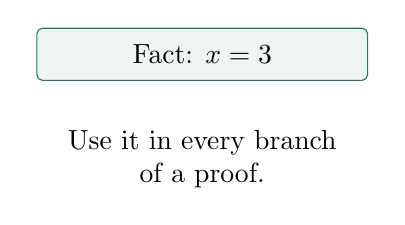
\begin{tikzpicture}
          \node[persistent, minimum width=4.2cm] (fact)
            {Fact: $x=3$};
          \node[below=5mm of fact, text width=4.2cm, align=center]
            {Use it in every branch\\of a proof.};
        \end{tikzpicture}
      \end{center}
    \end{column}
    \begin{column}{0.47\textwidth}
      \begin{center}
        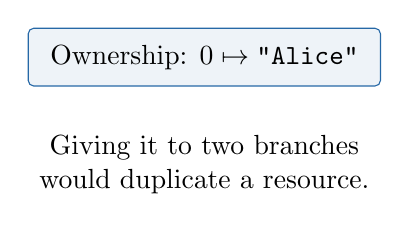
\begin{tikzpicture}
          \node[resource, minimum width=4.2cm] (cell)
            {Ownership: $0\mapsto\texttt{"Alice"}$};
          \node[below=5mm of cell, text width=4.2cm, align=center]
            {Giving it to two branches\\would duplicate a resource.};
        \end{tikzpicture}
      \end{center}
    \end{column}
  \end{columns}

  \vfill
  \begin{center}
    \large Can a proof assistant check both \kw{truth} and \kw{resource use}?
  \end{center}
\end{frame}

\begin{frame}{A second conjunction}
  \slidelead{A resource assertion $P:\Heap\to\PropCat$ says which owned heaps make $P$ true.}

  \begin{columns}[T,onlytextwidth]
    \begin{column}{0.46\textwidth}
      \minorhead{Additive conjunction}
      \[
        (P\land Q)(h) \quad\Longleftrightarrow\quad
        P(h)\land Q(h)
      \]
      Both claims inspect the \kw{same} resource.
    \end{column}
    \begin{column}{0.51\textwidth}
      \minorhead{Separating conjunction}
      \[
        \begin{aligned}
        (P\Sep Q)(h) \quad\Longleftrightarrow\quad
        \exists h_1,h_2.\;&h_1\disjoint h_2 \\
          {}\land\;&h=h_1\heapunion h_2\\
          {}\land\;&P(h_1)\land Q(h_2)
        \end{aligned}
      \]
      The claims receive \kw{disjoint} resources.
    \end{column}
  \end{columns}

  \begin{center}
    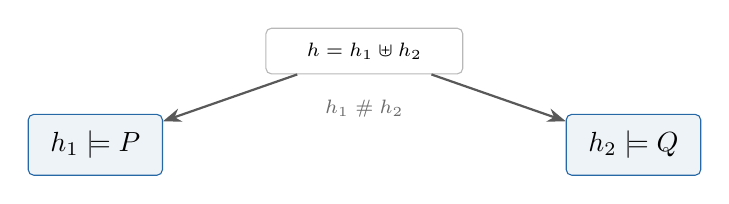
\begin{tikzpicture}[node distance=12mm]
      \node[pptbox, minimum width=2.5cm] (whole) {$h=h_1\heapunion h_2$};
      \node[resource, below left=5mm and 13mm of whole] (left) {$h_1\models P$};
      \node[resource, below right=5mm and 13mm of whole] (right) {$h_2\models Q$};
      \draw[pptarrow] (whole) -- (left);
      \draw[pptarrow] (whole) -- (right);
      \node[smallnote, below=2mm of whole] {$h_1\disjoint h_2$};
    \end{tikzpicture}
  \end{center}
\end{frame}

\begin{frame}{Two laws you can now predict}
  \slidelead{The algebra of $\Sep$ comes from splitting heaps.}

  \begin{columns}[T,onlytextwidth]
    \begin{column}{0.48\textwidth}
      \minorhead{Rearranging independent ownership}
      \keyeq{(0\mapsto A)\Sep(1\mapsto B)
        \;\Entails\;(1\mapsto B)\Sep(0\mapsto A)}
      Swap the two disjoint pieces.
    \end{column}
    \begin{column}{0.48\textwidth}
      \minorhead{Exclusive ownership}
      \keyeq{(0\mapsto A)\Sep(0\mapsto A)
        \;\Entails\;\false}
      One location cannot occur in both pieces.
    \end{column}
  \end{columns}

  \vfill
  \begin{center}
    \large This is the central idea of \kw{separation logic}.
  \end{center}
\end{frame}

\begin{frame}{The project in one sentence}
  \slidelead{MPSL is a small, kernel-checked laboratory for a resource logic.}

  \begin{center}
    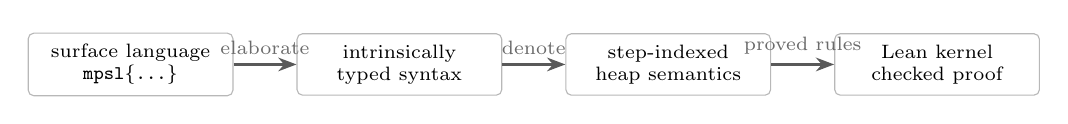
\begin{tikzpicture}[node distance=7mm and 8mm]
      \node[pptbox, minimum width=2.6cm] (surface) {surface language\\\texttt{mpsl\{...\}}};
      \node[pptbox, right=of surface, minimum width=2.6cm] (typed) {intrinsically\\typed syntax};
      \node[pptbox, right=of typed, minimum width=2.6cm] (sem) {step-indexed\\heap semantics};
      \node[pptbox, right=of sem, minimum width=2.6cm] (kernel) {Lean kernel\\checked proof};
      \draw[pptarrow] (surface) -- node[above,smallnote]{elaborate} (typed);
      \draw[pptarrow] (typed) -- node[above,smallnote]{denote} (sem);
      \draw[pptarrow] (sem) -- node[above,smallnote]{proved rules} (kernel);
    \end{tikzpicture}
  \end{center}

  \vspace{0.55cm}
  \begin{columns}[T,onlytextwidth]
    \begin{column}{0.31\textwidth}
      \minorhead{Language}
      Higher-order formulas, quantifiers, equality, $\Sep$, $\Always$, and $\Later$.
    \end{column}
    \begin{column}{0.31\textwidth}
      \minorhead{Semantics}
      Partial heaps, exclusive points-to, finite observations, and proved laws.
    \end{column}
    \begin{column}{0.31\textwidth}
      \minorhead{Proof mode}
      Named reusable and spatial contexts with explicit resource partitioning.
    \end{column}
  \end{columns}
\end{frame}

\begin{frame}[fragile]{A proof is resource bookkeeping}
  \begin{columns}[T,onlytextwidth]
    \begin{column}{0.53\textwidth}
\begin{lstlisting}[style=leancode]
example (P Q : Formula Nat String) :
    mpsl{ `P ∗ `Q } (*@$\Entails$@*) mpsl{ `Q ∗ `P } := by
  mintro h
  mdestruct h as hP hQ
  msep [hQ]
  · mexact hQ
  · mexact hP
\end{lstlisting}
    \end{column}
    \begin{column}{0.43\textwidth}
      \minorhead{After \texttt{mdestruct}}
      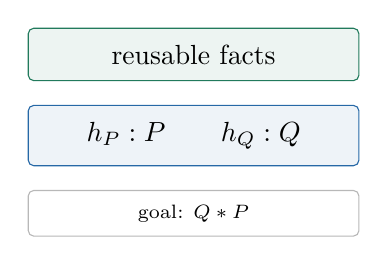
\begin{tikzpicture}
        \node[persistent, minimum width=4.2cm] (p) {reusable facts};
        \node[resource, below=3mm of p, minimum width=4.2cm] (s)
          {$h_P:P\qquad h_Q:Q$};
        \node[pptbox, below=3mm of s, minimum width=4.2cm] (g)
          {goal: $Q\Sep P$};
      \end{tikzpicture}

      \vspace{0.35cm}
      \texttt{msep [hQ]} sends $h_Q$ left and the remaining resource $h_P$ right.
    \end{column}
  \end{columns}

  \vfill
  \muted{Every tactic applies a proved semantic rule; it does not become part of the trusted logic.}
\end{frame}

% Speaker: This is the category-theoretic entry point. Prop is regarded as the
% preorder/category of propositions and implications.
\begin{frame}{A proposition observed at every precision}
  \slidelead{Replace one proposition by a coherent diagram of approximations.}

  Let $\omega=(\mathbb{N},\leq)$ and regard propositions and implications as a category:
  \[
    P : \omega^{\mathrm{op}} \longrightarrow \PropCat.
  \]

  \begin{center}
    \begin{tikzpicture}[node distance=15mm]
      \node[stage] (p0) {$P_0$};
      \node[stage, right=of p0] (p1) {$P_1$};
      \node[stage, right=of p1] (p2) {$P_2$};
      \node[stage, right=of p2] (p3) {$P_3$};
      \node[right=8mm of p3] (dots) {$\cdots$};
      \draw[pptarrow] (p1) -- (p0);
      \draw[pptarrow] (p2) -- (p1);
      \draw[pptarrow] (p3) -- (p2);
      \draw[pptarrow] (dots) -- (p3);
    \end{tikzpicture}
  \end{center}

  \keyeq{m\leq n \quad\Longrightarrow\quad P_n\Rightarrow P_m}

  \begin{center}
    $P_n$: ``$P$ survives observation at precision $n$.''
  \end{center}

  \vfill
  \muted{This is MPSL's \texttt{SProp}: a downward-closed predicate on $\mathbb{N}$.}
\end{frame}

\begin{frame}{Later is the shift of the diagram}
  \slidelead{No clock and no program execution: $\Later$ lowers precision by one.}

  \keyeq{(\Later P)_0=\true,
    \qquad (\Later P)_{n+1}=P_n}

  \begin{center}
    \begin{tikzpicture}[node distance=13mm]
      \node[stage] (t) {$\top$};
      \node[stage, right=of t] (p0) {$P_0$};
      \node[stage, right=of p0] (p1) {$P_1$};
      \node[stage, right=of p1] (p2) {$P_2$};
      \node[right=8mm of p2] (dots) {$\cdots$};
      \draw[pptarrow] (p0) -- (t);
      \draw[pptarrow] (p1) -- (p0);
      \draw[pptarrow] (p2) -- (p1);
      \draw[pptarrow] (dots) -- (p2);
      \node[below=6mm of t, smallnote] {precision 0};
      \node[below=6mm of p0, smallnote] {precision 1};
      \node[below=6mm of p1, smallnote] {precision 2};
      \node[below=6mm of p2, smallnote] {precision 3};
    \end{tikzpicture}
  \end{center}

  \vspace{0.45cm}
  \minorhead{Why does $P\Entails\Later P$ hold?}
  At level $0$, $\Later P$ is automatic. At level $n+1$, downward closure
  gives exactly the required map $P_{n+1}\Rightarrow P_n$.
\end{frame}

\begin{frame}{L\"ob induction is induction in disguise}
  \slidelead{A seemingly circular hypothesis is guarded by a strictly smaller index.}

  \[
    \inferrule
      {\Later P\Entails P}
      {\Entails P}
    \qquad\text{(L\"ob)}
  \]

  Fix a heap $h$.  We prove $P(h,n)$ for every $n$ by ordinary induction.

  \vspace{0.25cm}
  \begin{columns}[T,onlytextwidth]
    \begin{column}{0.47\textwidth}
      \minorhead{Base case: $n=0$}
      \[
        (\Later P)(h,0)=\true.
      \]
      The premise $\Later P\Entails P$ therefore proves $P(h,0)$.
    \end{column}
    \begin{column}{0.49\textwidth}
      \minorhead{Inductive step: $n\rightsquigarrow n+1$}
      \[
        (\Later P)(h,n+1)=P(h,n).
      \]
      The induction hypothesis supplies the left-hand side; the premise gives $P(h,n+1)$.
    \end{column}
  \end{columns}

  \vfill
  \begin{center}
    \large ``Assume $P$ later'' means ``assume $P$ at a smaller index.''

    \vspace{0.15cm}
    \scriptsize\muted{MPSL's \texttt{mlob ih} implements this rule. With spatial resources it guards
      $\Gamma_s\Wand P$, so the induction hypothesis cannot duplicate ownership.}
  \end{center}
\end{frame}

\begin{frame}{Finite agreement makes higher order safe}
  \slidelead{At precision $n$, assertions are compared only through level $n$.}

  \keyeq{P =_n Q
    \quad\Longleftrightarrow\quad
    \forall m\leq n,\; P_m\leftrightarrow Q_m}

  A function on assertions is required to be \kw{non-expansive}:
  \[
    P=_n Q \quad\Longrightarrow\quad F(P)=_n F(Q).
  \]

  \begin{center}
    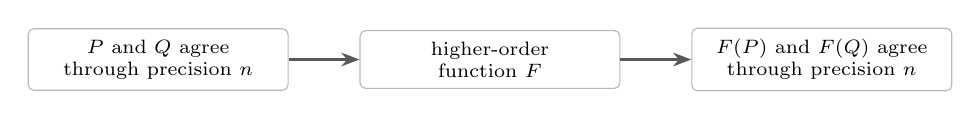
\begin{tikzpicture}[node distance=9mm]
      \node[pptbox, minimum width=3.3cm] (in) {$P$ and $Q$ agree\\through precision $n$};
      \node[pptbox, right=of in, minimum width=3.3cm] (fun) {higher-order\\function $F$};
      \node[pptbox, right=of fun, minimum width=3.3cm] (out) {$F(P)$ and $F(Q)$ agree\\through precision $n$};
      \draw[pptarrow] (in) -- (fun);
      \draw[pptarrow] (fun) -- (out);
    \end{tikzpicture}
  \end{center}

  \vfill
  \begin{center}
    $F$ cannot manufacture information at a precision it was not given.
  \end{center}
\end{frame}

\begin{frame}{What MPSL does---and deliberately does not do}
  \begin{columns}[T,onlytextwidth]
    \begin{column}{0.47\textwidth}
      \minorhead{Implemented}
      \begin{itemize}
        \item intrinsically typed higher-order DSL;
        \item affine separation logic over partial heaps;
        \item $\Always$, $\Later$, quantifiers, equality, and points-to;
        \item OFEs and non-expansive function spaces;
        \item sound named proof mode and InfoView rendering.
      \end{itemize}
    \end{column}
    \begin{column}{0.47\textwidth}
      \minorhead{Outside the current scope}
      \begin{itemize}
        \item program syntax and operational semantics;
        \item weakest preconditions and Hoare triples;
        \item invariants, ghost state, and generic resources;
        \item guarded fixed points and recursive predicates.
      \end{itemize}
    \end{column}
  \end{columns}

  \vfill
  \begin{center}
    \large The goal is a \kw{small, inspectable semantic core}, not a full Iris replacement.
  \end{center}
\end{frame}

\begin{frame}{Three ideas to take away}
  \vspace{0.4cm}
  \begin{enumerate}
    \item \textbf{Assertions can describe ownership, not only truth.}

      $P\Sep Q$ splits the available resource into disjoint pieces.

    \item \textbf{Step indexing is a diagram of finite approximations.}

      $\Later$ is its shift; L\"ob induction is ordinary induction on the index.

    \item \textbf{MPSL connects notation to a kernel-checked semantics.}

      Typed elaboration, proved logical laws, and a resource-aware proof mode form one checked pipeline.
  \end{enumerate}

  \vfill
  \begin{center}
    \Large\textcolor{PKURed}{Truth, ownership, and approximation---checked together.}
  \end{center}
\end{frame}

\begin{frame}
  \vspace{2.25cm}
  {\Huge\bfseries\textcolor{PKURed}{Thank You}\par}
  \vspace{0.45cm}
  {\Large Questions and Comments Welcome\par}
\end{frame}

\end{document}
